\documentclass{article}
\usepackage[utf8]{inputenc}

\usepackage{indentfirst}
\usepackage{biblatex}
\usepackage{amsmath}
\usepackage{graphicx}

\title{Sentiment Analysis Report}
\author{NGUYEN, Ngoc Gia Hy }
\date{\today}


\graphicspath{ {images/} }
\addbibresource{ref.bib}


\begin{document}

\maketitle

\section{Introduction}

With the explosive of the Internet in this digital age, more and more people easily access the Internet and share their opinions on social media (i.e., reviews, forum discussion, blogs and social networks). 
By analyzing or observing these opinions, individuals and organizations are easier in decision making. 
For instance, potential customers can know about advantages and drawbacks of a service before using by reading it's reviews from other users.
Businesses always want to know customers opinions to improve the quality of product in the next version or the next generation. 
However there are a lot of websites on the Internet, this leads to a difficulty to find or monitor the huge volume of opinionated text by manual methods.
Moreover, it is also known that human analysis may have some bias caused by  subjective opinions of human toward some services or products.

Instead of using manual methods, they become more interested in analyzing opinionated text automatically.
Therefore automated opinion mining and summarization systems are needed.
These systems can overcome the limitation of subjective opinion bias and shortage amount of opinionated text observing by human.
In the past decade, a considerable amount of research has been done in academia to build up these systems by solving the problem named Opinion Mining in Natural Language Processing~\cite{Liu10sentimentanalysis,Pang:2008:OMS:1454711.1454712}.
This report briefly describes Opinion Mining tasks.
Beside that, I also give a survey of about Aspect Based Sentiment Analysis, a subproblem of Sentiment Analysis which I intend to do in my thesis.

The remaining of this report is organized as follow.
Section~\ref{sec:sabackground} describes some background knowledge about Opinion Mining and Sentiment Analysis problem. 
Then Aspect Based Sentiment Analysis (ABSA) and its recent works are illustrated in section~\ref{sec:sbsa}. 
The next (section~\ref{sec:rpl})  is my research plans for Aspect Based Sentiment Analysis and the final one is Discussion section.

\section{Opinion Mining and Sentiment Analysis}
This section give some fundamental principles of Opinion Mining and Sentiment Analysis problem.
Firstly, opinion problem is defined to enable us to see structured form of  opinions in unstructured text data.
Secondly, I describe some tasks of Sentiment Analysis which are principle elements of building automated opinion mining and summarization systems.

\label{sec:sabackground}
\subsection{The problem of Opinion Mining}
According to Bing Liu~\cite{Liu2012}, opinions can be expressed about anything, e.g., a product, a service, an individual, an organization, an event, or a topic, by any person or organization.
An opinion is a quintuple, $(e_i, a_{ij}, oo_{ijkl}, h_k, t_l)$ where $e_i$ is the name of an entity, $a_{ij}$ is an aspect of $e_i$, $oo_{ijkl}$ is the orientation of the opinion about aspect $a_{ij}$ of entity $e_i$, $h_k$ is the opinion holder, and $t_l$ is the time when the opinion is expressed by $h_k$. 
The opinion orientation $oo_{ijkl}$ can be positive, negative or neutral, or be expressed with different strength/intensity levels. 
When an opinion is not toward any particular aspect, we denote it by using special aspect GENERAL.
A example below clearly illustrates the quintuple.

\textbf{Example 1}:
(Blog Posting) Posted by: bigXyz on Nov-4-2010: 
(1) I bought a Motorola phone and my girlfriend bought a Nokia phone yesterday. 
(2) We called each other when we got home. 
(3) The voice of my Moto phone was unclear, but the camera was good. 
(4) My girlfriend was quite happy with her phone, and its sound quality. 
(5) I want a phone with good voice quality. 
(6) So I probably will not keep it.

The goal of opinion mining is to extract four following quintuples in the example above:
\begin{itemize}
	\item (Motorola, voice\_quality, negative, bigXyz, Nov-4-2010)
	\item (Motorola, camera, positive, bigXyz, Nov-4-2010)
	\item (Nokia, GENERAL, positive, bigXyz's\_girlfriend, Nov-4-2010)
	\item (Nokia, voice\_quality, positive, bigXyz's\_girlfriend, Nov-4-2010)
\end{itemize}
We can easily recognise that each quintuple above describes orderly: entity, aspect, sentiment, opinion holder, and time corresponding to the definition $e_i, a_{ij}, oo_{ijkl}, h_k, t_l$ respectively. 

To achieve this goal, we have to solve the following tasks:
\begin{itemize}
	\item \textbf{Task 1: Entity extraction and grouping}: extract all entities in an opinionated document D and group synonymous entities into entity clusters. Each cluster indicates a unique entity $e_i$. For example, task 1 should extract three entities "Motorola", "Nokia", and "Moto" in example 1 and then generate two entity cluster "Motorola", "Nokia" in which "Motorola" and "Moto" are grouped.
	\item \textbf{Task 2: Aspect extraction and grouping}: extract all aspects and group synonymous aspects into aspect clusters. Each aspect cluster $a_{ij}$ indicates a particular aspect of $e_i$. For example, task 2 should extract three aspects “camera”, “voice”, and “sound” in example 1, and group “voice” and “sound” together as they are synonyms representing the same aspect.
	\item \textbf{Task 3: Opinion holder and time extraction}: extract name of holder and time in D. It is “bigXyz", “bigXyz's\_girlfriend", and Nov-4-2010 in the example.
	\item \textbf{Task 4: Aspect sentiment classification}: determine whether each opinion on an aspect of an entity is positive, negative or neutral. 
	\item \textbf{Task 5: Opinion quintuple generation}: generate all quintuples as form $(e_i, a_{ij}, oo_{ijkl}, h_k, t_l)$ like 4 quintuples above.
\end{itemize}


\subsection{Opinion Tasks}
This section give brief 
\subsubsection{Aspect-Based Opinion Summary}

To give a general view about a product or a service, most opinion applications should automatically extract quintuples from a large number of opinions expressed by different holders and then generate a summary based on entities and aspects.
This task is known as Aspect-Based Opinion Summary ( or feature-based opinion summary)~\cite{Hu:2004:MSC:1014052.1014073, Liu:2005:OOA:1060745.1060797}.
Figure~\ref{fir:abos} below illustrates a structured summary which is proposed by 	Minqing Hu~\cite{Hu:2004:MSC:1014052.1014073}. 
Although structured summary at figure~\ref{fir:abos} can be visualized by using bar chart or pie chart, some researchers~\cite{Beineke04anexploration,COIN:COIN417,Ku2016,Seki06opinion-focusedsummarization,Stoyanov:2006:PSC:1610075.1610123} studied opinion summarization in the tradition fashion that give a quick overview about product as a short text summary. 
For instance, "Most people like voice quality in Cellular phone 1".

\begin{figure}[ht]
\centering
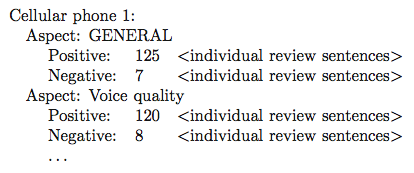
\includegraphics[width=0.65\textwidth]{AbOS}
\caption{Structured Summary}
\label{fir:abos}
\end{figure}

\subsubsection{Document Sentiment Classification}

Document sentiment classification is essentially a problem of text classification.
It determines whether a given document D is positive, negative, or neutral (predefined classes).
The task is also known as document-level sentiment classification because it considers the whole document as the basic information unit~\cite{Liu2012}.
With the assumption that the opinion document D expresses opinions on a single entity $e$ and the opinions are from a single opinion holder $h$, document sentiment classification generates only one quintuple $(e,GENERAL,oo,h,t)$. 

A common approach for document sentiment classification is based on supervised learning.
Input and output of document sentiment classification model is a pair (X, y) in which X is features vector extracted from document D, y is opinion label of document D (positive, negative, or neutral).
The model aims to find the relationship between input and output through training stage, and then predicts output given a new input in test stage.
Pang et al.~\cite{Pang:2002:TUS:1118693.1118704} did experiences with this supervised learning method and stated that unigrams (a bag of individual words) features perform well with either naive Bayesian, support vector machine model.
Moreover, instead of using different learning model, effective set of features are also considered. It contains Terms and their frequency (TF-IDF); Part of speech (POS); Opinion words and phrases; Negations; Syntactic dependency; sentiment WordNet; or emoticon dictionary.

Unsupervised learning method is another approach for document sentiment classification. 
Since opinion words and phrases are dominating indicators for sentiment classification, we can use their features for scoring in unsupervised learning method.
This method can be described as following three steps according to~\cite{DBLP:journals/corr/cs-LG-0212032}.
\begin{itemize}
	\item Step 1: extracts phrases containing adjectives or adverbs as adjectives and adverbs are good indicators of opinions.
	\item Step 2: estimates the semantic orientation of the extracted phrases using the pointwise mutual information (\textbf{PMI}).
	\item Step 3: given a review, the algorithm computes the average semantic orientation (\textbf{SO}) of all phrases in the review, and classifies the review as recommended if the average SO is positive, not recommended otherwise.
\end{itemize}
Although this method is simple, it performs well in various domains range from 84\% for automobile reviews to 66\% for movie reviews.
%TODO co nen them diem manh va yeu cua sentiment tren document ko

\subsubsection{Sentence Subjectivity and Sentiment Classification}
%TODO dinh nghia sentence subjectivity
According to Liu et al.~\cite{Liu2012}, a subjective sentence expresses some personal feelings, views or belief while objective sentence expresses some factual information about the world.
Almost objective sentences have no opinion.
Therefore determining whether a sentence is subjectivity or objectivity before using sentiment classification might boost performance of the system.
This subtask is often called as subjectivity classification in the existing literature~\cite{Hatzivassiloglou:2000:EAO:990820.990864, Pang:2005:SSE:1219840.1219855, Pang:2002:TUS:1118693.1118704, Wiebe:2004:LSL:1105596.1105598, Wilson:2004:JMY:1597148.1597270, COIN:COIN275, Yu:2003:TAO:1119355.1119372}. 
%TODO add citation

Essentially, sentence subjectivity and sentiment classification are similar to document sentiment classification.
The only difference one is the input unit (sentence instead of document), therefore the same document-level sentiment classification techniques can also be applied naturally to individual sentences.
Given a sentence $s$ and a assumption that $s$ expresses a single opinion from a single opinion holder, two sub-tasks are performed:
\begin{itemize}
	\item Subjectivity classification: determine whether $s$ is a subjective sentence or an objective sentence.
	\item Sentence-level sentiment classification: If $s$ is subjective, determine whether it expresses a positive, negative or neutral opinion.
\end{itemize}
These subtasks have two main advantages. 
Firstly, as mention above it filters out those sentences `contain no opinions. 
Secondly, after knowing about what entities and aspects we want to focus on, second task help us determine whether the opinions about the entities and their aspects are positive or negative. 

\subsubsection{Opinion Lexicon Expansion}
As mention above, opinion words and phrases are known as good features for not only supervised learning models but also unsupervised learning models.
This is due to the fact that the better features the model extract, the higher accuracy the model obtain.
In order to create and expand opinion word list, three main approaches have been introduced:
\begin{itemize}
	\item \textbf{Manual approach} usually use to collect opinion words and phrases as seeds before expanding them through other approaches. Although we may have a concise Opinion Lexicon (opinion words and phrases), it is very time consuming.
	\item \textbf{Dictionary based approach} usually use to expand Opinion Lexicon using dictionaries, WordNet~\cite{Miller90wordnet:an}, thesaurus~\cite{Mohammad:2009:GHS:1699571.1699591}, etc.
		 The main idea is bootstrapping. 
		 After collecting manually small set of opinion words and phrases, we expand this set by finding synonyms and antonyms in WordNet or thesaurus. 
		 This approach is very simple, but the approach is unable to find opinion words with domain and context specific orientations. For example, for a  phone speaker, if it is quiet, it is usually negative. 
		 However, for a car, if it is quiet, it is positive~\cite{Liu2012}. This problem is tackled by Corpus-based approach.
	\item \textbf{Corpus-based approach and sentiment consistency} usually use to expand Opinion Lexicon using syntactic or cooccurrence patterns and a large corpus. 
		The key idea is proposed by Hazivassiloglou and McKeown~\cite{Hatzivassiloglou:1997:PSO:976909.979640}. 
		The technique starts with a small set of opinion words, then a set of linguistic constraints or conventions on connectives is used to expand this word set. 
		For instance, conjunction AND usually have the same orientation. 
		With similar idea, recent works also consider neighboring sentences and pair (aspect, opinion word) to expand Opinion Lexicon. 
		Although preparing a huge corpus is a problem, this approach can overcome the problem of finding opinion words with domain and context specific orientations which is mentioned in Dictionary based approach.
\end{itemize}

\subsubsection{Other tasks}
Besides the problems mentioned above and Aspect Based Sentiment Analysis problems introduced in section~\ref{sec:sbsa}, there are two challenge  tasks and other minor tasks in opinion mining.

\textbf{Mining Comparative Opinions} relate to comparative sentences which express the comparison, similarities, or differences of more than one entity.
		Recent works~\cite{Dave:2003:MPG:775152.775226,Ding:2009:EDA:1557019.1557141, Ganapathibhotla:2008:MOC:1599081.1599112,Jindal:2006:MCS:1597348.1597400} as a whole use four types of comparative relations: non-equal gradable comparisons, equative comparisons, superlative comparisons, and non-gradable comparisons to meet the goal that generate comparative sextuples $(E_1, E_2, A, PE, h, t)$.
		$E_1,E_2$ are entities that is comparing based on aspect $A$.
		$PE (\in \{E1, E2\})$ is the prefered entity of the opinion holder h, and t is the time
		
\textbf{Opinion Spam Detection} is also a significant task in opinion mining.
		We all can see that a huge number of fake opinions (spam opinions) may affect critically to individual decision marking or product evaluation of business.
		Therefore, we should filter out these fake opinions before using other opinion evaluations.
		This task is investigated by some recent works~\cite{Jindal:2008:OSA:1341531.1341560,Jindal:2007:RSD:1242572.1242759,Lim:2010:DPR:1871437.1871557,Mukherjee:2011:DGR:1963192.1963240}.
		In generally, these works use rules and features such as human behaviors; relation between opinion text, mentioned entity and product information in order to detect spam opinions.
		
Besides, Opinion Mining also contains many meaningful tasks such as entity, opinion holder, and time extraction; objective expressions implying sentiments; grouping aspect expressions indicating the same aspects, mapping implicit aspect expressions to aspects, coreference resolution, and cross lingual opinion mining.

\section{Aspect Based Sentiment Analysis - ABSA}
\label{sec:sbsa}

In some cases, we want to know more detail opinions about which parts of product people are talking or are expressing opinions rather than the overall opinions.
For example, an positive opinionated document about a product does not mean that the holder like all parts of this product.
Maybe, the holder don't like some aspect	 but this does not affect to positive overall felling.
Although document-level sentiment classification is useful in many cases, it is not effective in this situation. 
To obtain these details, we need to go the aspect level.


As mention in the end of section \ref{sec:sabackground}, to obtain the aspect level, we have to perform 5 tasks orderly in order to generate quintuples $(e_i, a_{ij}, oo_{ijkl}, h_k, t_l)$.
In this section, I focus on task 2 and 4 named aspect extraction and aspect sentiment classification respectively because task 1 (entity extraction and grouping) is more related to another problem in Natural Language Processing named Named-entity recognition.
Moreover, task 3 and 5 are easily solved by extracting user informations and generating quintuples by task 2 and 4 results.

\subsection{Aspect Extraction}
% Introduction methods
Recent researches on aspect extraction mainly work on online reviews. Although there a lot of existing methods, we can divide into two categories: unsupervised method and supervised method. 
In supervised methods, by treating data as sequences like some NLP problems such as POS Tagging, Chunking, or Named Entity Recognition, researchers can apply sequence supervised learning models (CRF~\cite{Jakob:2010:EOT:1870658.1870759,Lafferty:2001:CRF:645530.655813} and HMM~\cite{Freitag00informationextraction,Jin:2009:NLH:1553374.1553435,Ding:2008:HLA:1341531.1341561}) to aspect extraction problem.

In unsupervised methods, Minqing Hu et al.~\cite{Hu:2004:MSC:1014052.1014073}  introduced a method consists of 2 steps to collect aspect words as much as possible. 
Firstly, frequent nouns and noun phrases are collected by counting the frequency of them.
This is due to the idea that the vocabulary usually converges when people comment on different aspects of a product.
Secondly, the model tries to collect infrequent nouns and noun phrases by exploiting the relationships or the occurrence between aspects and opinion words.
For instance, by exploiting the sentence "The pictures are absolutely amazing	", which contains "picture" aspect and "amazing" opinion word, we can easily extract "software" aspect in this sentence, "The software is amazing".
Ana-Maria Popescu~\cite{Popescu:2005:EPF:1220575.1220618} improved step 1 by trying to remove noun phrases that may not be product aspects/features such as "of scanner", "scanner has", "scanner comes with" of "scanner" class.

Topic modeling is considered as second method in unsupervised models.
Titov and McDonald~\cite{Titov:2008:MOR:1367497.1367513} proposed multi-grain topic models to discover local rateable aspects. 
Such discovered aspect is an unigram language model.
Although this language model is not easy to interpret aspects, it can automatically group the words that have the same aspect.
However, their method can not separate aspects and opinion words.
Therefore, Lin and He~\cite{Lin:2009:JSM:1645953.1646003} and Mei et al.~\cite{Mei:2007:TSM:1242572.1242596} proposed join topic-sentiment model, and positive, negative sentiment model respectively in order to separate these aspects and opinion words.
Zhao et al.~\cite{citeulike:9605702} proposed a MaxEnt-LDA hybrid model to discover both aspect words and aspect-specific opinion words to help separate aspects and opinion words.

\subsection{Aspect Sentiment Classification}
Although we can use sentence-level classification method in this problem, this method is quite difficult to deal with mixed opinion in a sentence.
For instance, if we focus on "Apple" aspect in a following sentence "Apple is doing very well in this terrible economy", the sentiment should be positive. 
However, if we focus on "economy", the sentiment should be negative.
Therefore, we need some phrase-level methods that mainly focus on phrases which contain considered aspects.
Like aspect extraction problem, we can use two main methods to tackle this problem, supervised and unsupervised methods.

In unsupervised learning methods, recent works use an opinion lexicon, i.e.. a list of opinion words and phrases, and a set of rules to determine the sentiments in opinions in a sentence~\cite{Ding:2008:HLA:1341531.1341561,Hu:2004:MSC:1014052.1014073}. 
This method is called lexicon-based method.
The method consists of 4 steps.
Firstly, opinion words and phrases are marked and scored with sentiment score, e.g. +1 for positive words and -1 for negative words.
Secondly, we adjusts sentiment scores of opinion words and phrases by handling opinion shifters which may change opinion orientations, e.g. not, never, none, ....
Thirdly, we continuously adjusts sentiment score by handling but-clauses.
Finally, an opinion aggregation function is applied to the resulting opinion scores to determine the final sentiment on each aspect.
The final sentiment of an aspect is calculated by sentiment scores of aspect's context opinion words and phrases.
Although, this method is simple and perform well in many cases, we need to prepare a large opinion lexicon to cover all type of opinions. 


In supervised learning methods, they treat aspect sentiment classification as target-dependence sentiment analysis.
In that problem, target is considered as aspect, dependence is context words.
Jiang et al.~\cite{Jiang:2011:TTS:2002472.2002492} first emphasizes the importance of targets by showing that 40\% of sentiment analysis errors are caused by not considering them in classification.
They incorporate 7 target-dependence features and other sentiment features into Support Vector Machine model and obtain a significant improvement.
Dong et al.~\cite{dong2014adaptive} apply the idea of target-dependence to Recursive Neural Network (RNN) on dependency tree.
The RNN model composes abstract representation of the context words orderly, from farthest to nearest in the tree, and then it composes representation of target words at final step.
This means that if we have multi targets in one sentence, each one have a individual way to compose informations of their context words based on their position. 
Moreover, closest context words, which contain a major meaning to target words, are mainly considered by the model.
By using two type of tree structures: dependency and constituent trees, Hai and Shirai~\cite{DBLP:conf/emnlp/NguyenS15} proposed PhraseRNN which make the abstract representation of target and dependence words richer.
In stead of using semantic relations between aspect and context words like previous works, Duyu Tang et al.~\cite{DBLP:journals/corr/TangQFL15} uses two LSTM networks running towards to target words from left and right respectively. 
The final states of both networks are concatenated and the prediction is made at the target word.
Duyu Tang et al.~\cite{DBLP:journals/corr/TangQL16} and Peng Chen et al.~\cite{D17-1048} take the advantage of Deep Memory Network and Attention Mechanism to achieve state-of-the-art result.

\section{Discussion}
\label{sec:disc}
This report gives an overview about some main Opinion Mining tasks.
These tasks are still challenges and attract researchers around the world in recent years.
Therefore, an annual opinion mining competition named SeemEval is opened in order to make a playground for researchers in this field.
Beside that, the report also presents a literature review of aspect sentiment classification in recent years.
Recent works show that supervised learning especially deep learning is a potential method to tackle aspect sentiment classification problem.




\printbibliography

%TODO bold nhung ky hieu e, h, bang $e$
\end{document}
